\section{Motivation}

In this section, we first study the typical shuffle characteristics (\ref{shuffle pattern}), and then spot the opportunities to achieve shuffle optmization (\ref{observation})
\subsection{Characteristic of Shuffle} \label{shuffle pattern}

In large scale data parallel computing, enormous datasets are partitioned into pieces to fit the memory of each node since the very beginning of MapReduce\cite{mapreduce} model.
Meanwhile, complicated application procedures are divided into steps. The successor steps take the output of ancestors as input to do the computation. Shuffle occurs when each successor needs 
part of data from all ancestors' output. In order to provide a clear illustration, we define those computing on each partition of data in one step as a task. For tasks that generate shuffle output, we call
them map task. For tasks that consume shuffle output, we call them reudce tasks. Note that one task may have both shuffle data generation and consumption in modern DAG framework. These tasks contain characteristic of both map task and reduce task. But these tasks won't change the behavior of shuffle. To avoid ambiguity, in the following paper, we will only use term of map task to represent those who produce shuffle output, and reduce task to represent those who consume shuffle output.

Shuffle is designed to achieve an all-to-all data blocks transfer among nodes in the cluster. It exists in both MapReduce models and DAG computation models.

The overview process of shuffle is presented in Figure \ref{fig:shuffle_process}. Shuffle mainly contains two phases itself: \textit{Data Partition} and \textit{Data Transfer}. For \textit{Data Partition}, each map task will partition the result data (key, value pair) into several buckets according to the partition function.
The bucket number equals to the number of tasks in the next step. When the map tasks finish, all the shuffle output data will be written into local persistent storage for fault tolerance \cite{mapreduce, spark}.
\textit{Data Transfer} can be further divided into two parts: \textit{Shuffle Write} and \textit{Shuffle Read}. \textit{Shuffle Write} starts after execution of map tasks and intermediate tasks. Partitioned data will  be stored on disk during \textit{Shuffle Write}. \textit{Shuffle Read} starts at the beginning of reduce tasks. These tasks will fetch the data that belong to their corresponding partitions from both remote nodes and local storage.

In short, shuffle is loosely coupled with application context and it's I/O intensive.

Since the intensive I/O operation is triggered during a shuffle, this can introduce a significant latency to the application. Reports show that, 60\% of MapReduce jobs at Yahoo
and 20\% at Facebook are shuffle intensive workloads\cite{shufflewatcher}. For those shuffle intensive jobs, the shuffle lantency may even dominate Job Completion Time. 
For instance, a MapReduce trace analysis from Facebook shows that shuffle accounts for 33\% JCT on average, up to 70\% in shuffle intensive jobs\cite{managing}.
Meanwhile, the completion time of shuffle correlates with the performance of storage devices, network and even applications. 
This variation may bring a huge challenge for operators to find the correct configuration of the DAG framework.
\begin{figure}
	\centering
	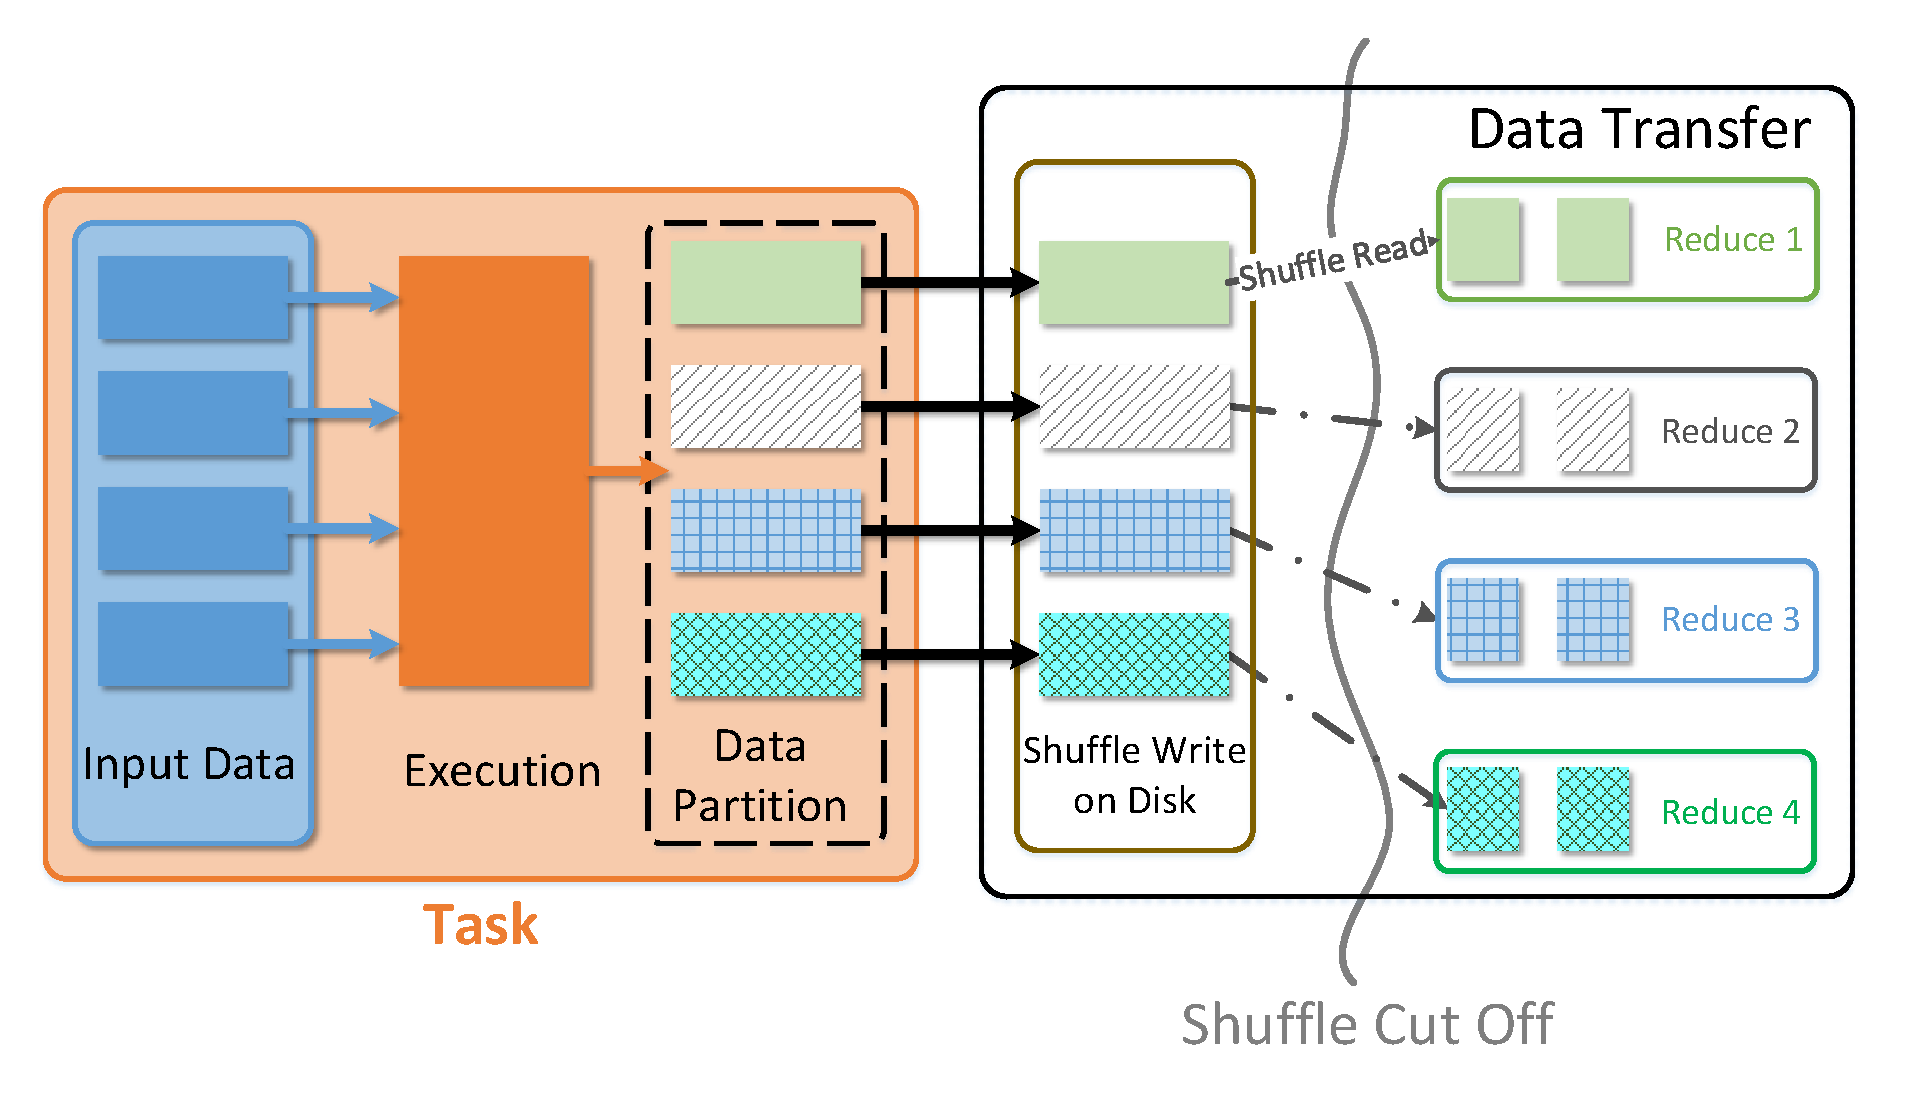
\includegraphics[width=\linewidth]{fig/shuffle_process}
	\caption{Shuffle Overview}
	\label{fig:shuffle_process}
\end{figure}

\subsection{Observations} \label{observation}
Of course, shuffle is unavoidable in a DAG computing process. But \textbf{\textit{can we mitigate or even remove the overhead of shuffle?}} To find the answers, we run some representative applications on a Spark in a 5 m4.xlarge Aamzon EC2 cluster. We then capture and plot the CPU utilization, I/O throughput and tasks execution information of each node. Take the trace in Figure \ref{fig:util} as an example, which is captured during one Spark GroupByTest job. This job has 2 rounds of tasks for each node. We mark the 'Execution' phase in the figure from the launch time of the first task of this node to the execution finish timestamp of the last one. The 'Shuffle Write' phase is marked from the timestamp of the begining of the first partitioned data write. The 'Shuffle Read and Execution' phase is marked from the start of the first reduce launch timestamp.
Figure \ref{fig:util} contains data, including two stages connected by one shuffle. By analyzing the trace combing with Spark, we propose following observations.
% \begin{figure*}
% 	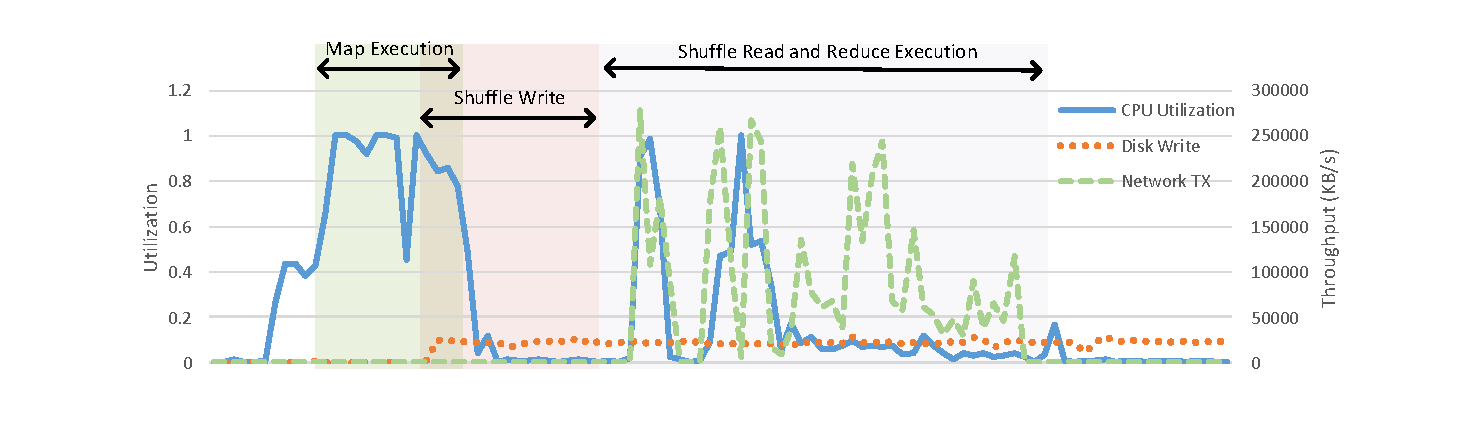
\includegraphics[width=\textwidth]{fig/util}
% 	\caption{CPU utiliazation and I/O throughput of a node during a Spark single shuffle application}
% 	\label{fig:util}
% \end{figure*}

\begin{figure}
	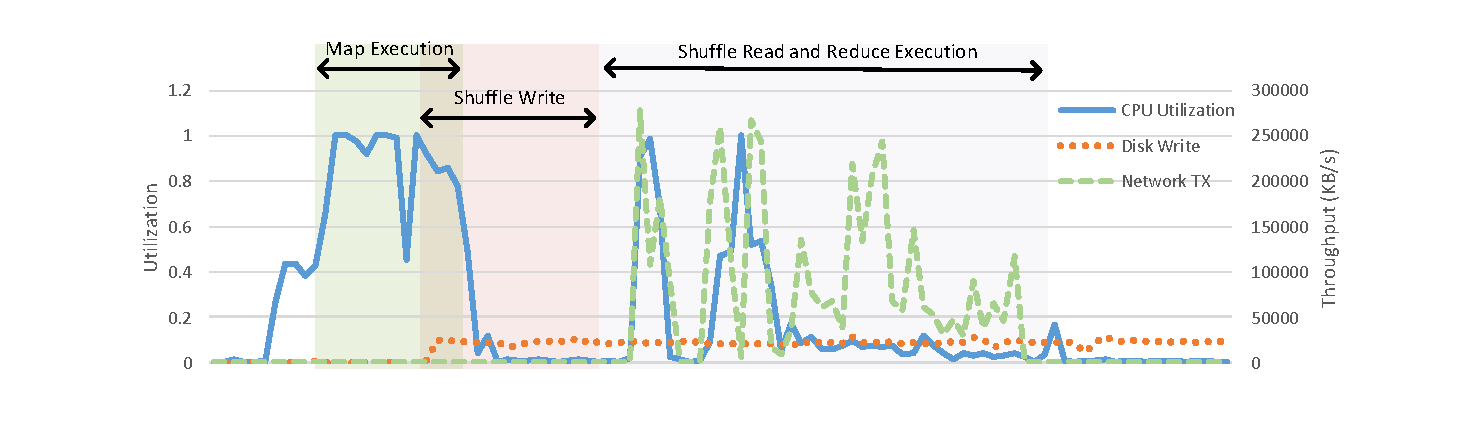
\includegraphics[width=\linewidth]{fig/util}
	\caption{CPU utiliazation and I/O throughput of a node during a Spark single shuffle application}
	\label{fig:util}
\end{figure}

\subsubsection{Multi-rounds tasks in each stages}\label{multi}
Both experience and DAG framework manuals recommend that multi-rounds execution of each stage will benefit the performance of applications.
For example, Hadoop MapReduce Tutorial \cite{hadooptutorial} suggests that \textit{10-100 maps per-node} and \textit{0.95 or 1.75 $\times$ no. of nodes $\times$ no. of maximum container per node} seem to be the right level of parallelism. Spark Configuration also recommends 2-3 tasks per CPU core in the cluster\cite{sparkconf}.
We have two rounds of tasks in job of Figure \ref{fig:util} to process about 70GB data. Figure \ref{fig:util} shows that the second phase of shuffle -- \textit{Data Transfer} will start until the reduce stage starts.
But the shuffle data will become available as soon as the execution of one task is finished. Though in the context of Spark, the reduce task can do computation while fetching data, the uncontrolled network congestion may still hurt the performance. However, if the destination of the shuffle output of each task is aware, the property of multi-rounds can be leveraged to do \textit{Data Transfer} ahead of reduce stage.

\subsubsection{Tight Copule between Shuffle and Computation}
Another information we get from the trace is that shffle should be decoupled from task which is a execution unit in both Spark and Hadoop MapReduce. In general, CPU and memory are binded as a schedule slot in DAG resource scheduler. When a task is scheduled to a slot, it won't release until it reaches the end of task. In Figure \ref{fig:util}, the resource of Spark executor will be realsed at the ending of 'Shffle Write'.
But CPU becomes idle almost as soon as the 'Exectuion' is finished. On the other hand, shuffle is I/O intensive job. It doesn't involved CPU and application context. If the shffle can be decopled from task, the slot can be relased after 'Execution' phase. The early release can benefit other tasks to achieve better overall performance of the DAG framework.

\subsubsection{Variance of I/O Performance}
When we look into the performance of disk and network in our test case, there is huge variance. Since we use the standard EBS as our backend storage for the EC2 instances, the I/O performance of the disk is poor. 
At the same time, the bandwidth of each instance is not specified from Amazon. But the utilization in Figure\ref{fig:util} refers that the bandwidth is about 300Mbps. In this case, the bottleneck of shuffle is disk, which introduces a significant latency for the application. Vice versa, in some cases, the congestion of network may also become the bottleneck of shuffle\cite{varys}. The uncertainty about the I/O performance causes a huge challenge for optimizing the DAG computing in the cluster. For network latency, the most we can do is to mitigate the transfer delay. As for disk write, we believe it's not necessary for today's cluster. Recall that the persistence of shuffle data is used only for reduce fault tolerence, but the mean time to failure(MTTF) for a server is counted in the scale of year\cite{tachyon}. The MTTF is exponential comparing with the duration of a shuffle, so we believe the disk write is unnecessary in today's data center. 

\subsubsection{Relatively Small Size of Shuffle Data}\label{shufflesize}
In order to accelearate computation, Spark will put all the input data set for a task into memory. Comparing to the input dataset, size of shuffle data is relatively small. We present two typical applications on Spark to show the relationship between shuffle data comparing with the input dataset in Figure \ref{fig:shuffle_size}. Although TeraSort\cite{terasort} is known as a shuffle intensive job, in a 10GB input TeraSort, the shuffle size is less than 3GB. When it's mapped to a 5-nodes cluster, it only takes about 500MB memory (\~25\% of input size for each node) to cache the shuffle data in memory. The data reported in \cite{makingsense} also shows that the amount of data shuffled is less than input data, by as much as a factor of 5-10. This is another reason that disk should not be involved in the whole shuffle procedure.


Based on these observations, it's straightforward to come up with an optimization that use memory to store the shuffle data and overlap the I/O operations of shuffle
by leveraging multi-rounds property of DAG computing. In order to achieve this optimization, we have to decouple shuffle from task and 
perform pre-fetch as soon as each output of map task and intermediate task is available. But is this feasible? We try to answer this question
in the following sections.
